%!TEX root = ../thesis.tex

\chapter{Methods}
\label{cha:methods}

In this chapter we are going to explain the different methods developed during this thesis.
First, we are going to explain the backbone architecture used during the entire thesis.
Then, we are going to explain how we train a CNN model to track points.
The last section will explain how metric learning works and how we have used it.

\section{Backbone Architecture}
\label{sec:methods:backbonearchitecture}

The objective of this thesis has been to obtain a deep learning model which is capable of, given a point per instance, being able to predict its segmentation through all the videos.
As it is usual on the literature, current best performing deep learning models for computer vision tasks (and more precisely in segmentation) use fully convolutional neural networks.
These models perform convolution operations over the input which is usually an image.

During the development of this thesis, we have used as a backbone architecture the DeepLab~\deeplab{} model for semantic segmentation.
This model is fully convolutional and it is based on the ResNet~\resnet{} architecture which was used for image classification.
The DeepLab~\deeplab{} model applies a sequence of convolutional layers to the input image, and instead of a classifier, plugs an Atrous Spatial Pyramid Pooling (also defined in~\deeplab{}) at the very last part of the architecture to obtain a segmentation mask.
%what does is to keep the convolutional layers from ResNet~\resnet and add at the end some deconvolutional operations to obtain as an output a mask instead of an object classifier.
Doing this allows the model to be fully convolutional and free of the constraint about the input image size.

The ResNet architecture is based on layers with residual connections.
\figref{backbonearchitecture:resnetblock} illustrates how each bottleneck layer block is built.
Each layer applies some convolutional operations to the input and then adds this result to the original input as a residual.

\begin{figure}[h]
  \centering
  \adjincludegraphics[trim={{.5\width} 0 0 0}, clip, width=.5\textwidth]{figures/resnet/block_deeper.pdf}
  \caption{ResNet~\resnet{} residual block architecture. }
  \label{fig:backbonearchitecture:resnetblock}
\end{figure}

For a more detailed description of the whole architecture of the DeepLab~\deeplab{} convolutional neural network see \tabref{backbonearchitecture:deeplabarch}, where two versions used are described: ResNet50 and ResNet101.
The architecture takes as input images of size $512 \times 512$ and outputs the input size downsampled by $8$ both in height and width.
Also, note that the number of output channels is 2048, so this output can be used directly, or a header can be plugged.
A header can be any group of layers that perform a task. Some examples could be a group of fully connected layers that can perform a classification, of a group of convolutional layers that reduce the dimensionality.
In the scenario of this thesis, a header made of a single convolutional filter with kernel size 1 have been used in order to test a dimensionality reduction.
% \ToDo{Explain what a header is} can be plugged to reduce the dimensionality (in the case of classification, reduce the dimensionality to the number of classes).
Because of these, this architecture is very versatile and easy to use with images.

\newcommand{\blocka}[2]{\multirow{3}{*}{\(\left[\begin{array}{c}\text{3$\times$3, #1}\\[-.1em] \text{3$\times$3, #1} \end{array}\right]\)$\times$#2}
}
\newcommand{\blockb}[3]{\multirow{3}{*}{\(\left[\begin{array}{c}\text{1$\times$1, #2}\\[-.1em] \text{3$\times$3, #2}\\[-.1em] \text{1$\times$1, #1}\end{array}\right]\)$\times$#3}
}
\begin{table}[h]
  \centering
  \begin{tabular}{c|c|c|c}
    \toprule
    layer name & output size & 50-layer & 101-layer \\
    \midrule
    conv1 & 256$\times$256 & \multicolumn{2}{c}{7$\times$7, 64, stride 2}\\
    \midrule
    \multirow{4}{*}{conv2\_x} & \multirow{4}{*}{128$\times$128} & \multicolumn{2}{c}{3$\times$3 max pool, stride 2} \\\cline{3-4}
      &  &  \blockb{256}{64}{3} & \blockb{256}{64}{3} \\
      &  &  &\\
      &  &  &\\
    \hline
    \multirow{3}{*}{conv3\_x} &  \multirow{3}{*}{64$\times$64}    & \blockb{512}{128}{4}  & \blockb{512}{128}{4}\\
      &  &  &\\
      &  &  & \\
    \hline
    \multirow{3}{*}{conv4\_x} & \multirow{3}{*}{64$\times$64}  & \blockb{1024}{256}{6}  & \blockb{1024}{256}{23} \\
      &  &  &\\
      &  &  & \\
    \hline
    \multirow{3}{*}{conv5\_x} & \multirow{3}{*}{64$\times$64}  &  \blockb{2048}{512}{3}  & \blockb{2048}{512}{3}\\
      &  &  &\\
      &  &  & \\
    \bottomrule
  \end{tabular}
  \caption{Architectures for DeepLab~\deeplab{} using residual blocks.
    Building blocks are shown in brackets (see also \figref{backbonearchitecture:resnetblock}), with the numbers of blocks stacked.
  }
  \label{tab:backbonearchitecture:deeplabarch}
\end{table}

In the original ResNet architecture downsampling with stride 2 was performed at layers \textit{conv3\_1}, \textit{conv4\_1} and \textit{conv5\_1}.
On DeepLab, the downsampling with stride 2 is only performed at \textit{conv3\_1}.
In contrast, in \textit{conv4\_x} and \textit{conv5\_x} all the convolutions are performed with dilation $2$ and $4$, respectively.
The dilated convolution was presented in~\dilatedconv{} and supports expansion of the receptive field without loss of spatial resolution.


\section{Tracking}
\label{sec:methods:tracking}

In order to track points through a video sequence, one possible approach is to regress the point position in an image using a heatmap.
The point representation is inspired by~\hourglass{} which used heatmaps to predict keypoints positions.
In our experiments, we are going to use the DeepLab ResNet architecture described in \secref{methods:backbonearchitecture} plus an additional module, a PSP~\pspnet{} module that will reduce the output to a single channel image.
This output can be trained to predict the point representation as a gaussian heatmap % using a pyramid scene parsing.\ToDo{Reformulate text}
% This will allow us to regress a heatmap representation of a point
using the Mean Squared Error loss function.

The heatmap is built using the coordinate of a point $p = (p_x, p_y)$ and computing a guassian around this point.
In \equref{tracking:heatmap} is shown how to build a heatmap $\mathcal{H}$ which allows some customization with the parameter $\sigma$ which is the spreadness of the sigma.
Note that the values of the heatmap are bounded between $[0, 1]$.
To observe a graphical example, in \figref{tracking:pointrepresentation} there is a point annotated on an image and the resulting heatmap.

\begin{equation}
  \mathcal{H}(x, y) = \exp \left[ -4 \log(2) \frac{ (x - p_x)^2 + (y - p_y)^2 }{ \sigma^2 } \right]
  \label{eq:tracking:heatmap}
\end{equation}

\begin{figure}[h]
  \centering
  \begin{subfigure}{.5\textwidth}
    \centering
    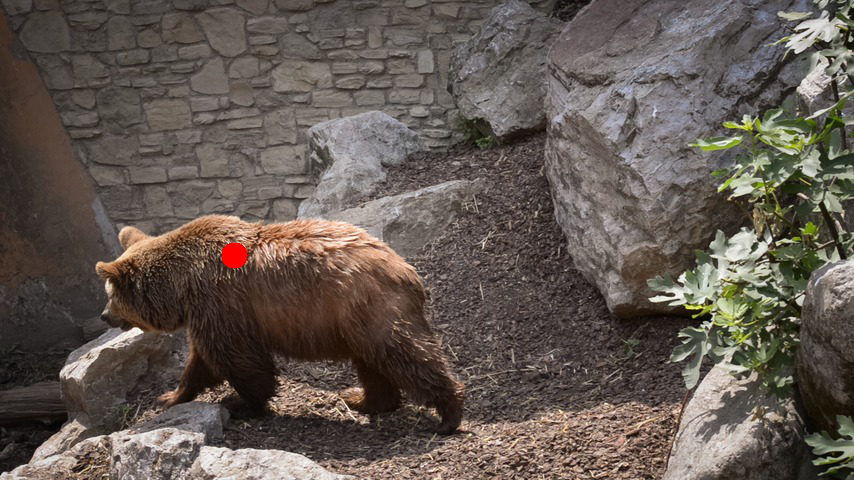
\includegraphics[width=.8\linewidth]{figures/methods/heatmaps/image_point.png}
  \end{subfigure}%
  \begin{subfigure}{.5\textwidth}
    \centering
    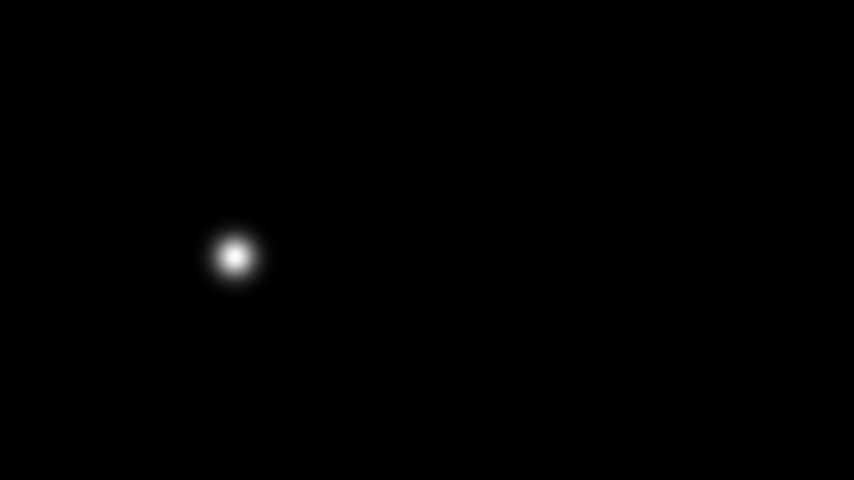
\includegraphics[width=.8\linewidth]{figures/methods/heatmaps/heatmap.png}
  \end{subfigure}
  \caption{
  Point representation.
  \textbf{Left}: Image with the annotated points (image resolution $854 \times 480$ pixels).
  \textbf{Right}: Heatmap to represent the point with $\sigma = 32$ pixels. }
  \label{fig:tracking:pointrepresentation}
\end{figure}

The strategy to train a model that tracks a point given in the first frame will be the same used in OSVOS~\osvos{}.
% TODO: Explain VOC
First is used a model pretrained on semantic segmentation which have learned the representation of all the classes appearing at PASCAL~\pascal{}.
Then this model is finetuned over the first frame of one sequence.
As we only have a single image, some data augmentation is required to enrich the training data and don't overfit on a single image.
Finally we will test each sequence's model with the rest of the frames and extract the predicted tracked point as the coordinate of the heatmap's maximum.
% with Visual Object Classes over the first frame of each sequence.
% Adding some data augmentation to enrich the training, we will test each sequence models with the rest of the frames and extract the maximum of the predicted heatmap as tracked object.

\section{Metric Learning with Triplet Loss}
\label{sec:methods:metriclearning}

Another approach to track a point in a video sequence could consist on training a model which outputs an embedding for each pixel that can be meaningful to obtain instance segmentation.
In order to obtain a good embedding, metric learning has been used.
Metric learning performs the task of learning a good embedding representation using distance comparison.
% distance function over objects, which in our case, the objects are embeddings.\ToDo{Reformulate}

One way to apply metric learning is using a Triplet Loss which was first introduced in~\metriclearning{}.
One famous implementation of this Triplet Loss was used in FaceNet~\facenet{} where they train a model to embed face images and predict similarity between them.

The objective of the Triplet Loss consists on learning a distance difference between triplets of points.
The triplet consists on three points that are called: anchor, positive and negative.
It must fill the condition that the label of the anchor and the positive point are the same, while the label of the negative is different.
The objective of the Triplet Loss is to push the distance of the anchor and positive points to be closer than the distance between the anchor and negative by some margin $\alpha$.
In \figref{tripletloss:visualization} a diagram about the learning procedure is shown.

\begin{figure}[h]
  \centering
  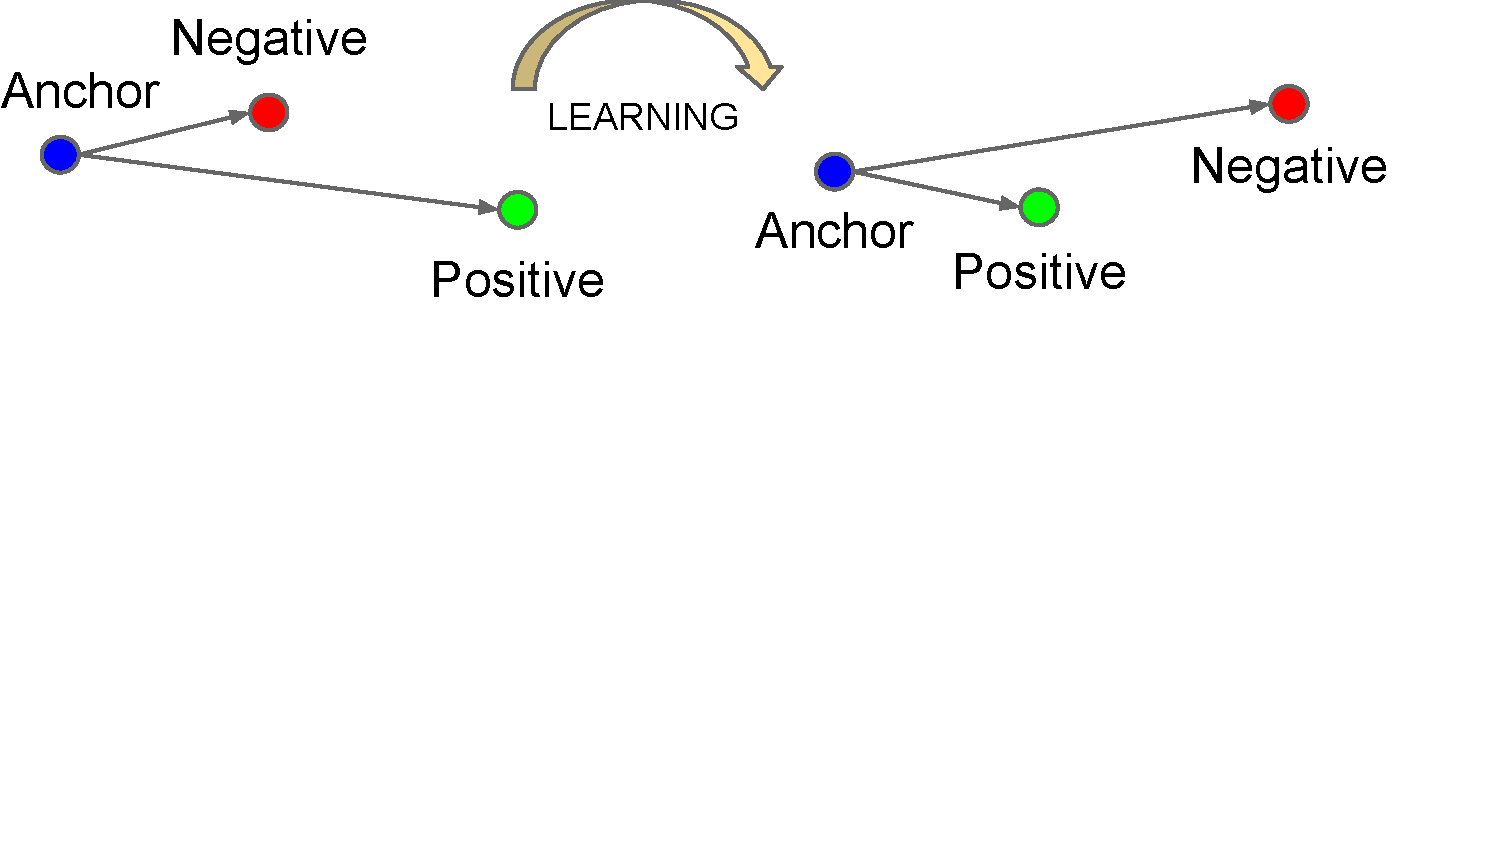
\includegraphics[trim=1cm 10cm 2.5cm 0cm, width=0.7\linewidth]{figures/methods/triplet_loss/triplet_viz.pdf}
  \caption{
    Graphical representation of Triplet Loss learning.
  Figure extracted from~\facenet{}. }
    \label{fig:tripletloss:visualization}
\end{figure}

In our scenario, we use DeepLab~\deeplab{} explained in detail in \secref{methods:backbonearchitecture}.
We use a model that is pretrained for semantic segmentation, and we use the full network except the last classification part which predicts the pixels class.
By default, this model given an image of size $H \times W$ output a features map of size $H' \times W' = \frac{H}{8} \times \frac{W}{8}$ with $2048$ dimensions.
A convolutional head can be plugged to reduce this dimensionality to a lower dimension $D$ which may lead to a better embedding.

Before giving the equations of the Triple Loss, we define the following notation.
Let $\mathcal{I} \in \mathbb{R}^{H \times W}$ be the input image of size $H \times W$.
The output size of the model will be $H' \times W' = \frac{H}{8} \times \frac{W}{8}$ and the output embedding will be $\mathcal{X} = \{x_i\}^{H' \times W'}$ where $x_i \in \mathbb{R}^D$ is the i-th output pixel embedding.
Let the Convolutional Neural Network be the embedding model $f(\mathcal{I}; \Theta)$ which computes the embedding from a single image:

\begin{equation}
  \mathcal{X} = f(\mathcal{I}; \Theta)
\end{equation}

When training the model,
only the mask of a single object is available , so the learning only pushes the embeddings of one instance at each time.
% there is available the ground truth mask of one object instance in the image.
When the image is forwarded through the model and the embeddings are computed, $N$ triplets of pixels are sampled.
For each triplet, two pixels belonging to the mask are sampled and assigned as anchor and positive pixels ($x_a$ and $x_p$ respectively).
Finally, a pixel not belonging to the mask is sampled and assigned as negative pixel $x_n$.

\begin{equation}
  \label{eq:tripletloss:1}
  \mathcal{L}_{triplet} = \sum_i^N \max \left( d(x_a^{(i)}, x_p^{(i)}) - d(x_a^{(i)}, x_n^{(i)})  + \alpha, 0 \right)
\end{equation}

The $\alpha$ term on the Triplet Loss is the margin used to enforce the minimum difference between the distance of positive pairs and negative pairs.
$d$ is the distance function, which in our case the $l^2$ norm is used.
So \equref{tripletloss:1} will end up as follows:

\begin{equation}
  \label{eq:tripletloss:2}
  \mathcal{L}_{triplet} =
	\sum_i^N \max \left(
		\|x_a^{(i)} - x_p^{(i)}\|_2 - \|x_a^{(i)} - x_n^{(i)}\|_2  + \alpha,
		0 \right)
\end{equation}

This learned embedding can be very useful for example to implement a second approach for tracking.
This can be done by computing the similarity between the embedding of the pixel to track with respect all the pixels in the future frames.
The tracked point can be extracted from the most similar.
% A similarity between pixel's embedding in the next frame and the embedding of the point to track in order to obtain its location on the next frame.


% At some point we tried to implement 2 triplet loss.
% Explain the precedure for far/close pixels.

\section{From Embeddings to Segmentation}
\label{sec:methods:embeddingsegmentation}

Once we have learned a good embedding for each pixel of the image, the embedding can not give us directly the segmentation of every instance.
As our approach will consist in tracking a point for every instance in the video sequence, an already annotated pixel will be provided.
We are going to call this pixel keypoint and its associated embedding $x_k \in \mathbb{R}^D$.
This point can come from the ground truth, from tracking or from another frame annotation.

In order to obtain the segmentation for multiple instances in an images given a keypoint for each instance, we can compute the distance of every pixel embedding against all keypoint embeddings.
Then, every pixel will be assigned to the label of the closest keypoint embedding only if this distance is lower than a threshold $\gamma$, otherwise will be assigned to background.
All of these can be formulated mathematically taking into account and image embedding $\mathcal{X}~=~\{x_i\}^{H \times W}$ with $N$ instances and each instance with a keypoint embedding $x_k^{(n)}$.
Every keypoint will have a label $m_k^{(n)} \in [1, N]$ and label $0$ will belong to the background.
The distance map for every image will be:

\begin{equation}
  \mathcal{D}_i = min_n \left( d(x_i, x_k^{(n)}) \right)
\end{equation}

Then the prediction label can be computed as follows:

\begin{equation}
  \mathcal{M}_i = \begin{cases}
      \arg\min_n d(x_i, x_k^{(n)}) & \mathcal{D}_i \leq \gamma \\
      0 & \mathcal{D}_i > \gamma
   \end{cases}
\end{equation}

All these steps can be visualized in \figref{instancesegmentation} where the ground-truth mask and a keypoint per each dog instance, the distance map of the embeddings against the keypoint embedding and finally the predicted mask are displayed.

\begin{figure}[h]
  \centering
  \instancesegmentation{1}
  \instancesegmentation{2}
  \instancesegmentation{3}
  \caption{Example of instance segmentation procedure given a point per instance.
  \textbf{Left}: Ground truth annotation of the instance and keypoint given.
  \textbf{Middle}: Distance map of the every pixel's embedding versus keypoint embedding (higher intensity means lower distance, dark means higher distance).
  \textbf{Right}: Predicted mask once applied the thresholding. }
  \label{fig:instancesegmentation}
\end{figure}
